In this section, we try to test the performance of online projection under various settings. 
\subsection{Quadratic cost}
We set $\beta = 0.5$, and $f_t(x) = \| A_t x - y_t\|_2^2$, where $A_t$ is a random $d \times d$ matrix with fixed condition number (default set to 10), and $y_t \in \mathcal{Y} \subset \mathbb{R}^d$, and the diameter of $\mathcal{Y}$ is fixed (default set to 10). We vary the number of dimension $d$ for the problem, for each dimension, we run 10 trials, the result is shown in Fig. \ref{fig: cr_vs_dim}.  
\begin{figure}[h!]
	\centering
	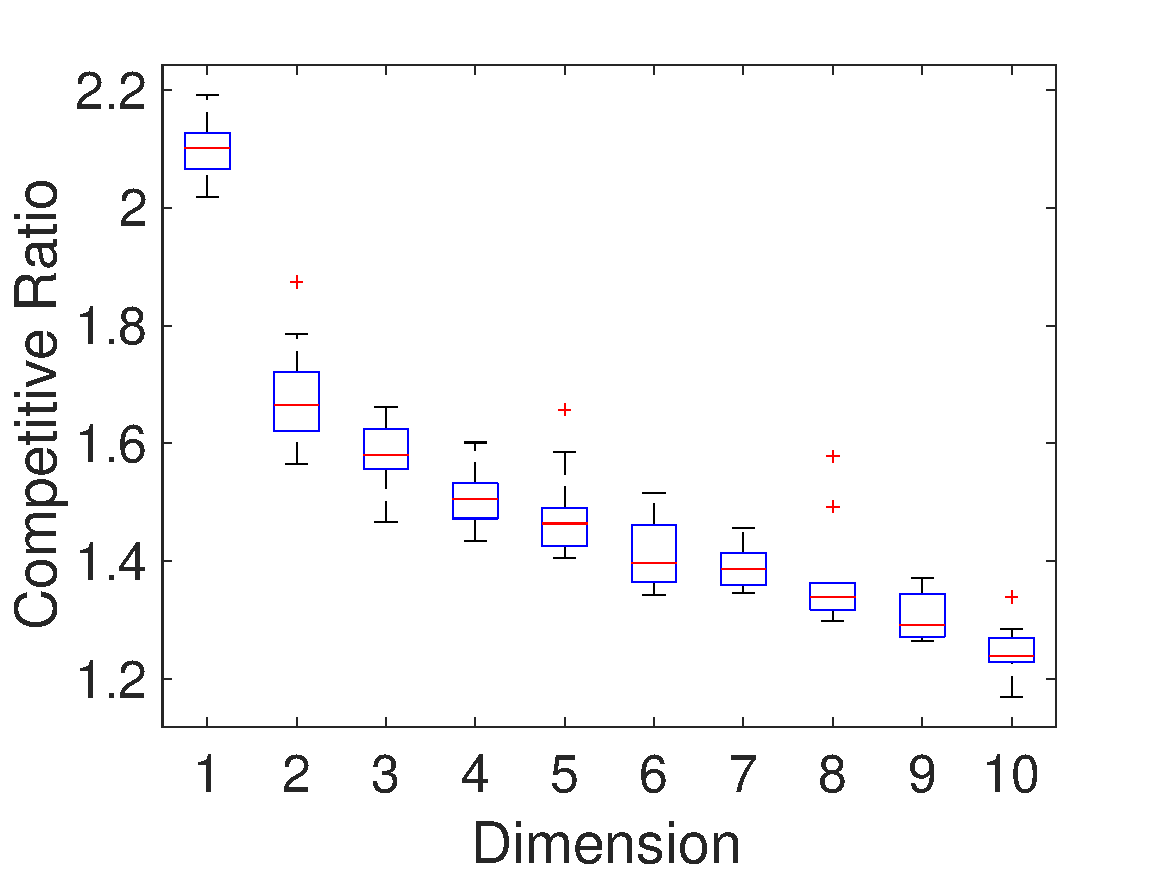
\includegraphics[width=.5\textwidth]{CR_vs_dimension}
	\caption{Competitive ratio against dimension while keeping the diameter of the feasible set constant}
	\label{fig: cr_vs_dim}
\end{figure}
Fig. \ref{fig: cr_vs_dim} shows that, surprisingly, the competitive ratio of Algorithm \ref{alg: online-projection} decreases as the dimension of the problem increases. 

\subsection{Linear cost}
We set $\beta = 0.5$, and $f_t(x) = \| A_t x - y_t\|_2$, where $A_t$ is a random $d \times d$ matrix with fixed condition number (default set to 10), and $y_t \in \mathcal{Y} \subset \mathbb{R}^d$, and the diameter of $\mathcal{Y}$ is fixed (default set to 10). We vary the number of dimension $d$ for the problem, for each dimension, we run 10 trials, the result is shown in Fig. \ref{fig: cr_vs_dim_lin}.
 \begin{figure}[h!]
	\centering
	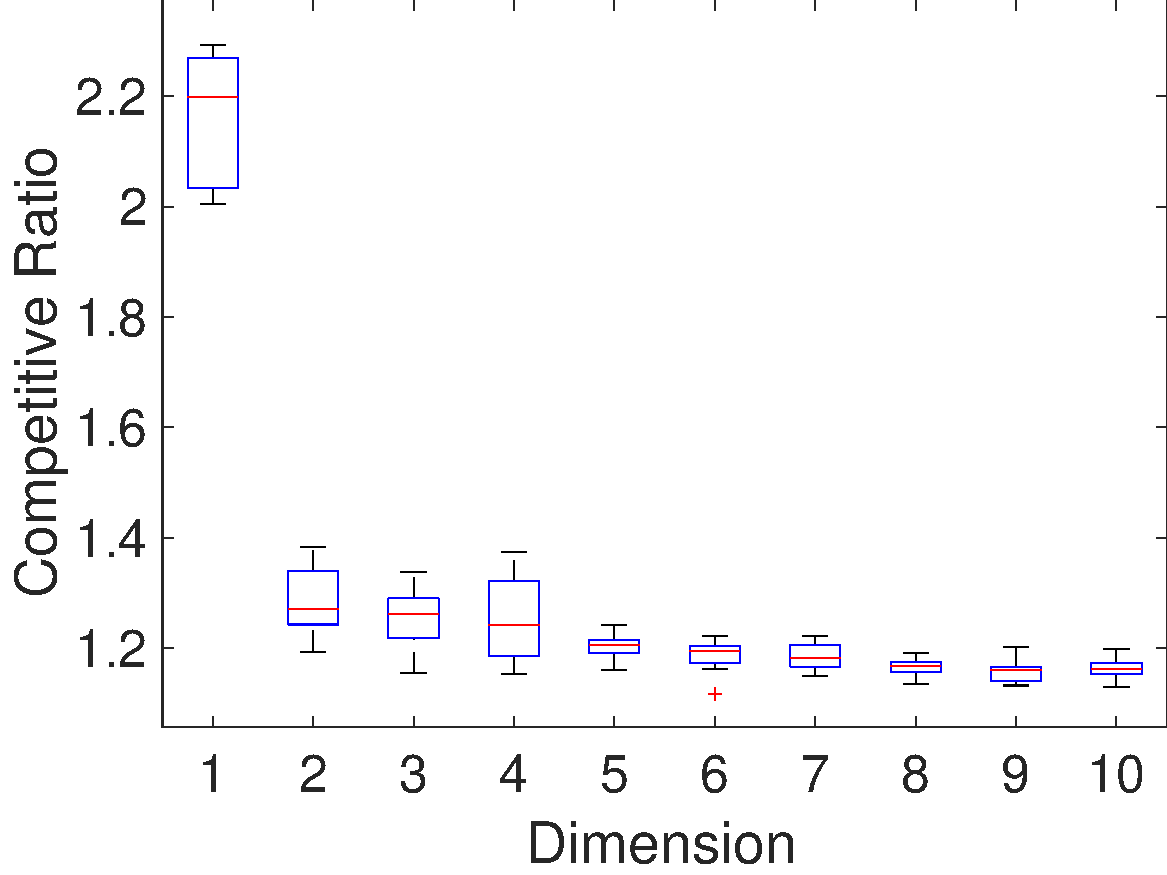
\includegraphics[width=.5\textwidth]{CR_vs_dimension_lin}
	\caption{Competitive ratio against dimension while keeping the diameter of the feasible set constant}
	\label{fig: cr_vs_dim_lin}
\end{figure}